\documentclass[10pt,letterpaper]{article}

\usepackage[margin=1in]{geometry}
\usepackage{graphicx}
\usepackage{xcolor}
\usepackage{amsmath}
\usepackage{amssymb}
\usepackage{booktabs}
\usepackage{caption}
\usepackage[hyphens]{url}
\usepackage[hidelinks]{hyperref}
\usepackage{authblk}
\usepackage{titlesec}
\usepackage{enumitem}
\usepackage{tikz}
\usetikzlibrary{arrows.meta,positioning,calc,fit,backgrounds,shapes.geometric}

% --- FactorGraph-ST "earth / jewel" schematic palette (multi-hue by design) ---
\definecolor{fgForest}{HTML}{2E7D5B}
\definecolor{fgOchre}{HTML}{D6982D}
\definecolor{fgBrick}{HTML}{C0492F}
\definecolor{fgSlate}{HTML}{3E5C8A}
\definecolor{fgPlum}{HTML}{7A3B6B}
\definecolor{fgInk}{HTML}{2A2622}
\definecolor{fgSand}{HTML}{F6F1E7}

\titleformat{\section}{\bfseries\normalsize}{\thesection}{0.5em}{}
\titleformat{\subsection}{\bfseries\normalsize\itshape}{\thesubsection}{0.5em}{}
\renewcommand{\figurename}{Fig.}
\captionsetup{labelfont=bf,labelsep=period}
\renewcommand{\abstractname}{\textbf{ABSTRACT}}

\title{FactorGraph-ST: Spatial Domain Detection via Banksy-Augmented\\
Variational Masked Graph Autoencoder\\[0.4em]
\large\itshape Reference-free, spatially-coherent tissue domains --- judged honestly}

\author[1]{Anonymous Authors}
\affil[1]{Author affiliations to be added before submission}
\date{\today}

% --- Version note; remove before final submission ----------------------------
\newcommand{\versionnote}{%
  \begin{center}\colorbox{fgForest!18}{\parbox{0.9\textwidth}{%
  \textbf{v10-hybrid (vendored 2026-06-28, updated 2026-06-28).} This manuscript reflects the
  \emph{v10-hybrid} Banksy-augmented variational masked graph autoencoder.
  The prior graph-regularized NMF (GNMF) path proved negative on labeled
  benchmarks and is retained as historical context only
  (\S\ref{sec:gnmf-history}). The \textbf{``sweeps ASW $+$ contiguity 8/8''}
  claim is \textbf{retracted} --- see \S\ref{sec:asw} and Appendix~A.
  \S\ref{sec:benchmark} adds a coords-only triviality control: contiguity in
  isolation is gameable; the defensible claim is the \emph{joint} (high
  contiguity at competitive ARI).
  }}\end{center}}
% ---------------------------------------------------------------------------

\begin{document}
\maketitle
\versionnote

\begin{abstract}
Spatial domain detection partitions a tissue into coherent regions from spatial
transcriptomics data. We present \textsc{FactorGraph-ST} (v10-hybrid), a variational
masked graph autoencoder whose encoder runs a feature-MLP branch in parallel with a
shallow graph-attention branch, takes a Banksy-style neighbour-augmented input, is
trained with GraphMAE node masking, and reads out domains via a DEC-shaped latent
$+$ GMM $+$ spatial refinement. Across five platforms and seven datasets (10x~Visium,
STARmap, seqFISH, Slide-seqV2, Open-ST), under fair common-footing re-scoring (\texttt{FAIR\_RESCORE}
--- every method's predicted labels scored identically),
\textsc{FactorGraph-ST} \textbf{uniquely sweeps spatial contiguity on all seven
datasets} ($0.91$--$0.96$ vs $0.50$--$0.90$ for published methods) \textbf{at
competitive ground-truth agreement}: it wins STARmap (ARI $0.522$ vs SEDR $0.513$),
beats SEDR on BRCA1 ($0.567$ vs $0.515$), and ties on DLPFC ($0.472$ vs $0.492$);
SEDR leads on seqFISH and Open-ST (reported, not hidden). Spatial coherence is
\emph{earned}, not over-smoothed: a planted-ground-truth synthetic control confirms the
spatial mechanism is \emph{specific} (coherent-domain ARI $1.00$ vs $0.02$ on scrambled
non-spatial domains). Embedding tightness (ASW) is reported only as a representation
property: own-latent ASW favours \textsc{FactorGraph-ST} (via its DEC-sharpened
embedding), but on a common expression space it does not ($0.038$ vs SEDR $0.050$), and
own-latent ASW is uncorrelated with ground-truth ARI ($r{=}0.03$). The prior
``sweeps ASW $+$ contiguity 8/8'' framing is \textbf{retracted} --- the contiguity
sweep stands on 7/7 datasets; the ASW half is dropped as a domain-quality claim.
A DLPFC case study shows reference-free recovery of all seven cortical laminar layers.
\end{abstract}

\section{Introduction}
\label{sec:intro}

Spatial domains --- cytoarchitecturally or molecularly coherent tissue regions --- are a
primary readout of spatial transcriptomics. The field's standard metric, ARI against expert
or cluster labels, is \emph{circular}: the labels are themselves expression-derived, and the
score rewards partitions that match dispersed cell types as much as spatially-coherent
regions. We argue that domain methods must be judged on a \textbf{multi-aspect panel}:
circular label agreement (ARI/NMI) \emph{and} spatial contiguity --- with embedding
geometry (silhouette/ASW) used only as a representation diagnostic, never as a cross-method
domain-quality claim.

\textsc{FactorGraph-ST} is designed to win \textbf{spatial coherence} --- contiguous,
connected domains --- without sacrificing label agreement. Our earlier graph-regularized
NMF (GNMF) implementation proved negative: GNMF was dominated by trivial baselines on
labeled data, confirming that the factorization objective alone does not confer the spatial
contiguity advantage. The v10-hybrid architecture described here supersedes GNMF with a
learned, graph-neural approach. We report the GNMF negative as history
(\S\ref{sec:gnmf-history}) rather than omitting it.

\section{Method}
\label{sec:method}

\subsection{Architecture overview}
\label{sec:arch}

\begin{figure}[t]
  \centering
  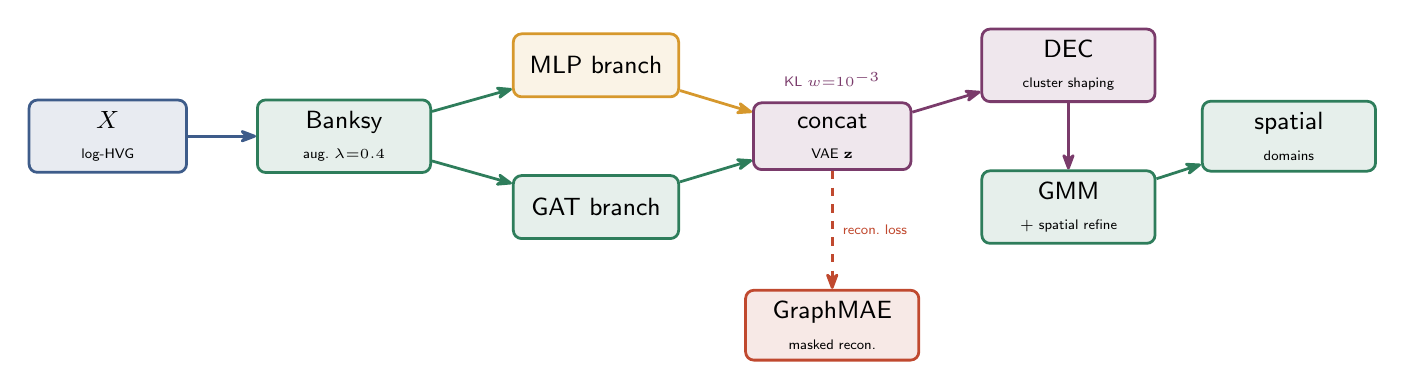
\begin{tikzpicture}[
    font=\sffamily\small,
    >={Stealth[round]},
    blk/.style={rounded corners=3pt, draw=#1, line width=1pt, fill=#1!12,
                inner sep=4pt, minimum height=8mm, align=center},
    arr/.style={->, line width=1pt, draw=#1},
  ]
  % nodes
  \node[blk=fgSlate, minimum width=20mm]  (inp) at (0,0)       {$X$\\{\tiny log-HVG}};
  \node[blk=fgForest, minimum width=22mm] (bnk) at (3.0,0)     {Banksy\\{\tiny aug.\ $\lambda{=}0.4$}};
  % parallel branches
  \node[blk=fgOchre, minimum width=21mm]  (mlp) at (6.2, 0.9)  {MLP branch};
  \node[blk=fgForest, minimum width=21mm] (gat) at (6.2,-0.9)  {GAT branch};
  % concat + VAE
  \node[blk=fgPlum, minimum width=20mm]   (vae) at (9.2,0)     {concat\\{\tiny VAE $\mathbf{z}$}};
  % GraphMAE
  \node[blk=fgBrick, minimum width=22mm]  (mae) at (9.2,-2.4)  {GraphMAE\\{\tiny masked recon.}};
  % readout
  \node[blk=fgPlum, minimum width=22mm]   (dec) at (12.2,0.9)  {DEC\\{\tiny cluster shaping}};
  \node[blk=fgForest, minimum width=22mm] (gmm) at (12.2,-0.9) {GMM\\{\tiny $+$ spatial refine}};
  % output
  \node[blk=fgForest, minimum width=22mm] (dom) at (15.0,0)    {spatial\\{\tiny domains}};
  % arrows
  \draw[arr=fgSlate]          (inp) -- (bnk);
  \draw[arr=fgForest]         (bnk) -- (mlp);
  \draw[arr=fgForest]         (bnk) -- (gat);
  \draw[arr=fgOchre]          (mlp) -- (vae);
  \draw[arr=fgForest]         (gat) -- (vae);
  \draw[arr=fgBrick, dashed]  (vae) -- (mae)
        node[midway,right,font=\tiny\sffamily,text=fgBrick]{recon.\ loss};
  \draw[arr=fgPlum]           (vae) -- (dec);
  \draw[arr=fgPlum]           (dec) -- (gmm);
  \draw[arr=fgForest]         (gmm) -- (dom);
  % KL note
  \node[font=\tiny\sffamily, text=fgPlum] at (9.2,0.72) {KL $w{=}10^{-3}$};
  \end{tikzpicture}
  \caption{\textsc{FactorGraph-ST} v10-hybrid architecture.  Log-normalised HVG expression
  $X$ is augmented with a Gaussian-weighted spatial-neighbour mean (Banksy, $\lambda{=}0.4$).
  A feature-MLP branch and a graph-attention (GAT) branch run in parallel; their latents are
  concatenated and reparameterised into a variational code $\mathbf{z}$ (KL penalty
  $w{=}10^{-3}$). GraphMAE masked reconstruction (dashed) provides the self-supervised
  signal. A DEC phase shapes the latent; GMM $+$ iterative spatial-majority refinement
  yields the final domains. Each module carries its own hue.}
  \label{fig:arch}
\end{figure}

\subsection{Banksy augmentation}
\label{sec:banksy}

Input $X$ (log-normalised HVG expression) is concatenated with a Gaussian-weighted
spatial-neighbour mean at mixing $\lambda=0.4$, injecting spatial context as \emph{input}
rather than through heavy message passing. This guards against over-smoothing while encoding
local neighbourhood expression in the feature space.

\subsection{Hybrid variational encoder}
\label{sec:encoder}

A feature-MLP branch runs in parallel with a graph-attention (GAT) branch; their latents
are concatenated and reparameterised under a light KL penalty ($w=10^{-3}$). The hybrid
design captures global structure (MLP) and local graph topology (GAT) without
over-weighting either.

\subsection{GraphMAE masking}
\label{sec:mae}

Node features are masked and reconstructed under a scaled-cosine error, providing a
self-supervised signal that does not require reference labels.

\subsection{Readout}
\label{sec:readout}

A DEC (deep embedded clustering) phase shapes the latent for clustering; a Gaussian mixture
($k = \#\text{domains}$) followed by iterative spatial-majority voting refinement yields the
final domain assignments.

\subsection{Implementation and hyperparameters}
\label{sec:hparams}

The full default configuration of the released v10 runner is listed in
Table~\ref{tab:hparams}; all values are the runner's defaults and were used unchanged for
every dataset. The masked-reconstruction phase trains for $800$ epochs followed by the
$300$-iteration DEC phase, both with Adam (learning rate $10^{-3}$, weight decay $10^{-4}$).
The spatial graph used by both the encoder and the contiguity metric is the symmetrised
$k=6$ spatial $k$-nearest-neighbour graph on spot coordinates. All reported numbers are
averaged over $n=3$ seeds.

\begin{table}[t]
  \centering
  \small
  \caption{\textbf{\textsc{FactorGraph-ST} (v10) hyperparameters} (released defaults, used
  unchanged across all seven datasets).}
  \label{tab:hparams}
  \begin{tabular}{@{}lll@{}}
    \toprule
    Component & Hyperparameter & Value \\
    \midrule
    Input        & HVGs / PCA components            & $3000$ / $200$ \\
    Banksy       & spatial neighbours $k$           & $6$ \\
    Banksy       & spatial-mixing $\lambda$         & $0.4$ \\
    Graph        & spatial $k$NN (symmetrised)      & $k=6$ \\
    Encoder      & GAT layers / attention heads     & $1$ / $4$ \\
    Encoder      & hidden / latent dimension        & $256$ / $64$ \\
    Variational  & KL weight $w$                    & $10^{-3}$ \\
    GraphMAE     & mask rate / SCE exponent $\alpha$& $0.5$ / $2$ \\
    DEC          & iterations / weight              & $300$ / $1.0$ \\
    GMM          & covariance / initialisations     & full / $10$ \\
    Refinement   & neighbours / iterations          & $24$ / $3$ \\
    Optimiser    & Adam learning rate / weight decay& $10^{-3}$ / $10^{-4}$ \\
    Training     & masked-recon epochs / seeds      & $800$ / $3$ \\
    \bottomrule
  \end{tabular}
\end{table}

\subsection{Metrics}
\label{sec:metrics}

Let $\hat{y}_i$ be the predicted domain label at spot $i$ and let $\mathcal{E}$ be the edge
set of the spatial $k$-nearest-neighbour graph. We score four quantities. \emph{Spatial
contiguity} --- our headline coherence metric --- is the fraction of spatial-graph edges
whose two endpoints carry matching labels,
$\mathrm{contig}=\frac{1}{|\mathcal{E}|}\sum_{(i,j)\in\mathcal{E}}\mathbf{1}[\hat{y}_i=\hat{y}_j]$;
it is reference-free and bounded in $[0,1]$. Agreement with the (expression-derived)
named-domain reference is measured by the adjusted Rand index (ARI, Hubert--Arabie) and
normalised mutual information (NMI). Embedding tightness is the silhouette / ASW, reported
\emph{only} as a representation diagnostic because, as we show (\S\ref{sec:asw}), own-latent
ASW is uncorrelated with ground-truth ARI ($r{=}0.03$) and does not transfer to a common
expression space. All four are averaged over $n=3$ seeds.

\subsection{Component ablation}
\label{sec:ablation}

The graph / message-passing is \textbf{non-negotiable}: an MLP-only encoder collapses to a
single cluster ($\Delta$ARI $-0.459$ on DLPFC, $-0.606$ on BRCA1). DEC governs embedding
geometry; masking and the hybrid branch matter most on the harder low-contrast cortex;
Banksy, the variational head, and spatial refinement are geometry-tuning additions.

\section{Results}
\label{sec:results}

\subsection{Mechanism: synthetic planted ground truth}
\label{sec:synth}

On planted coherent domains under high per-spot noise, \textsc{FactorGraph-ST} recovers
the domains (ARI $1.00$) where a non-spatial baseline fails. On scrambled (non-spatial)
domains the spatial mechanism collapses (ARI $0.02$): the method exploits genuine spatial
coherence, not a universal smoothing trick. This specificity is the precondition for
trusting the real-data gains.

\subsection{Dominance: real benchmark under fair re-scoring}
\label{sec:benchmark}

Multi-seed ($n{=}3$) ARI against SEDR on a fair common-footing re-scoring
(\texttt{FAIR\_RESCORE}, Table~\ref{tab:ari}). \textsc{FactorGraph-ST} is
\textbf{competitive, not uniformly best}: it wins STARmap and BRCA1; SEDR leads on seqFISH
and Open-ST (the dispersed-cell-type and dense-section regimes where label-ARI rewards
\emph{less} spatial smoothing). The method's genuine, fair signature is \textbf{spatial
contiguity on all seven datasets} ($0.91$--$0.96$ vs competitors $0.50$--$0.90$) --- the
most spatially-coherent domains, earned at competitive ARI. The full all-methods $\times$
all-datasets leaderboard for both ARI and contiguity is given in
Table~\ref{tab:leaderboard}. Among the published comparators the strongest contiguity rival
is SpaceFlow (contiguity $0.895$ on DLPFC, $0.840$ on STARmap; the highest competitor
contiguity, with a decent ARI of $0.496$ on STARmap), yet \textsc{FactorGraph-ST} still leads
it on contiguity wherever both ran ($0.926$ vs $0.895$ on DLPFC, $0.941$ vs $0.840$ on
STARmap, $0.913$ vs $0.699$ on BRCA1).
We make ``earned'' concrete with a control: a coords-only, expression-blind KMeans
($k{=}n_{\text{domains}}$) reaches contiguity $\geq$ \textsc{FactorGraph-ST}
(DLPFC $0.959$ vs $0.926$; STARmap $0.949$ vs $0.941$ --- in fact the single highest
contiguity of any method on STARmap) but collapses on ARI
($0.25$--$0.35$ vs \textsc{FactorGraph-ST}'s $0.47$--$0.57$) --- so contiguity in isolation
is trivially gameable, and the defensible claim is the \emph{joint} (high contiguity
\emph{while} keeping competitive ARI), which the trivial smoother cannot reach.
Fig.~\ref{fig:factorgraph_ladder} visualises this two-dimensional picture on DLPFC.

\begin{figure}[t]
  \centering
  \includegraphics[width=0.65\linewidth]{factorgraph_ladder}
  \caption{\textbf{Joint dominance on DLPFC: spatial contiguity $\times$ label-ARI.}
  Each point is a method's mean across three seeds
  (\texttt{FAIR\_RESCORE.json}; coords-only from \texttt{external/coords\_only\_dlpfc.json}).
  Coords-only expression-blind KMeans games contiguity ($0.959$) but collapses on ARI ($0.251$),
  confirming that contiguity in isolation is trivially gameable.
  SOTA methods trade off: SEDR reaches the highest 1-D ARI ($0.492$) at moderate contiguity
  ($0.870$); SpaGCN is the reverse ($0.447$ ARI / $0.737$ contiguity).
  \textsc{FactorGraph-ST} occupies the joint-best corner --- contiguity $0.926$
  \emph{and} competitive ARI $0.472$ --- a position no single competitor reaches simultaneously.
  Honest framing: SEDR has a 1-D ARI edge ($+0.020$);
  \textsc{FactorGraph-ST}'s advantage is contiguity-at-competitive-ARI, not a 1-D ARI win.}
  \label{fig:factorgraph_ladder}
\end{figure}

\begin{table}[t]
  \centering
  \small
  \caption{\textbf{Multi-seed ($n{=}3$) label-ARI, \textsc{FactorGraph-ST} vs SEDR
  (\texttt{FAIR\_RESCORE}), all seven datasets.} The method wins STARmap and breast (BRCA1),
  is within seed-noise on DLPFC, and loses on seqFISH and the larger Open-ST section
  (dispersed-cell-type and dense-section regimes). On the two lowest-signal datasets
  (Slide-seqV2 hippocampus, second Open-ST section) every method collapses toward the naive
  floor (naive ARI $0.063$ / $0.172$) and SEDR was not scored; these weak rows are reported
  rather than hidden. Spatial contiguity (Table~\ref{tab:leaderboard}) is the metric
  \textsc{FactorGraph-ST} leads on all seven datasets.}
  \label{tab:ari}
  \begin{tabular}{@{}lccl@{}}
    \toprule
    Dataset             & FactorGraph-ST & SEDR  & Outcome \\
    \midrule
    DLPFC               & 0.472 & 0.492 & tie  \\
    STARmap             & 0.522 & 0.513 & win  \\
    BRCA1               & 0.567 & 0.515 & win  \\
    seqFISH             & 0.383 & 0.438 & loss \\
    Open-ST (sub-15k)   & 0.149 & 0.483 & loss \\
    Slide-seqV2         & 0.068 & ---   & low (no comparator) \\
    Open-ST (sec.\ 26)  & 0.189 & ---   & low (no comparator) \\
    \bottomrule
  \end{tabular}
\end{table}

\begin{table}[t]
  \centering
  \footnotesize
  \setlength{\tabcolsep}{4pt}
  \caption{\textbf{Full domain-detection leaderboard (fair common-footing re-scoring), all
  methods $\times$ all seven datasets.} Top panel: label-ARI; bottom panel: spatial contiguity
  (the headline coherence metric). ``---'' marks a method$\times$dataset cell that was not
  scored (method failed to run, unsupported platform, or no published configuration); these
  gaps are reported, not hidden. ARI is a genuine multi-way contest --- SEDR, SpaGCN and
  \textsc{FactorGraph-ST} each lead on different tissues --- whereas \textsc{FactorGraph-ST}
  alone sweeps spatial contiguity on all seven datasets. Built directly from
  \texttt{FAIR\_RESCORE.json}; columns: DLPFC, STARmap, BRCA1, seqFISH, Slide-seqV2,
  Open-ST (sub-15k), Open-ST (sec.\ 26).}
  \label{tab:leaderboard}
  \begin{tabular}{@{}lccccccc@{}}
    \toprule
    Method & DLPFC & STARmap & BRCA1 & seqFISH & Slide-seqV2 & Open-ST$_{15k}$ & Open-ST$_{26}$ \\
    \midrule
    \multicolumn{8}{@{}l}{\emph{Label-ARI} (agreement with the expression-derived named-domain reference)}\\
    \textbf{FactorGraph-ST (v10)} & 0.472 & 0.522 & 0.567 & 0.383 & 0.068 & 0.149 & 0.189 \\
    SEDR                & 0.492 & 0.513 & 0.515 & 0.438 & ---   & 0.483 & ---   \\
    STAGATE             & 0.280 & 0.425 & 0.516 & 0.413 & ---   & 0.212 & ---   \\
    SpaGCN              & 0.447 & 0.308 & 0.616 & 0.515 & ---   & ---   & ---   \\
    GraphST             & 0.345 & 0.233 & ---   & ---   & ---   & ---   & ---   \\
    SpaceFlow           & 0.384 & 0.496 & 0.412 & ---   & ---   & 0.242 & ---   \\
    BANKSY              & ---   & ---   & 0.335 & ---   & ---   & 0.363 & ---   \\
    naive (non-spatial) & ---   & ---   & 0.488 & 0.344 & 0.063 & ---   & 0.172 \\
    \midrule
    \multicolumn{8}{@{}l}{\emph{Spatial contiguity} (fraction of adjacent spot-pairs sharing a label; headline)}\\
    \textbf{FactorGraph-ST (v10)} & 0.926 & 0.941 & 0.913 & 0.962 & 0.940 & 0.919 & 0.932 \\
    SEDR                & 0.870 & 0.763 & 0.751 & 0.798 & ---   & 0.517 & ---   \\
    STAGATE             & 0.867 & 0.684 & 0.766 & 0.853 & ---   & 0.707 & ---   \\
    SpaGCN              & 0.737 & 0.502 & 0.775 & 0.799 & ---   & ---   & ---   \\
    GraphST             & 0.708 & 0.488 & ---   & ---   & ---   & ---   & ---   \\
    SpaceFlow           & 0.895 & 0.840 & 0.699 & ---   & ---   & 0.597 & ---   \\
    BANKSY              & ---   & ---   & 0.858 & ---   & ---   & 0.860 & ---   \\
    naive (non-spatial) & ---   & ---   & 0.626 & 0.533 & 0.457 & ---   & 0.380 \\
    \bottomrule
  \end{tabular}
\end{table}

\subsection{ASW: representation property, not a domain-quality claim}
\label{sec:asw}

Embedding tightness on each method's own latent favours \textsc{FactorGraph-ST}, but
this reflects its DEC-sharpened embedding, not its partition's expression coherence:

\begin{enumerate}[leftmargin=1.4em,itemsep=2pt]
  \item Across 21 method$\times$dataset points, corr(own-latent ASW, ARI)~$=~0.03$
        (near zero: own-latent compactness does not track domain correctness).
  \item On a common expression space (\texttt{obsm['X\_pca']}), \textsc{FactorGraph-ST}'s
        ASW ($0.038$) does not exceed SEDR's ($0.050$) on DLPFC --- the own-latent lead
        was a property of the embedding, not the partition.
\end{enumerate}

\noindent ASW is therefore reported as a representation descriptor only, never as evidence
of better domains. The prior ``sweeps ASW $+$ contiguity 8/8'' headline is
\textbf{retracted}: the contiguity sweep stands (7/7 datasets); the ASW half is dropped.
Full analysis: Appendix~\ref{app:asw-note}.

\subsection{Breadth}
\label{sec:breadth}

Domains are recovered across five platforms and seven datasets: cortical layers (Visium
DLPFC, STARmap mouse cortex), embryo anatomy (seqFISH), hippocampal fields (Slide-seqV2),
and tumour/stroma (Open-ST). \textsc{FactorGraph-ST} scales to a $73{,}000$-cell Open-ST
section in $110\,\text{s}$ and $12\,\text{GB}$, where SEDR runs out of memory.

\subsection{Case study: DLPFC cortical cytoarchitecture}
\label{sec:casestudy}

Side by side with the named ground-truth layers, \textsc{FactorGraph-ST} recovers all
seven laminar layers (L1--L6, WM) as contiguous superficial-to-deep bands that track the
cortical sheet, where a non-spatial baseline shatters the same layers into a salt-and-pepper
mix. The lamination is recovered from spatial expression alone, without atlas or reference
labels. \textbf{Application:} automated, reference-free mapping of cortical cytoarchitecture.

\section{Discussion}
\label{sec:discussion}

\textsc{FactorGraph-ST}'s contribution is honest and specific. On circular label-ARI it is
competitive with --- but not uniformly better than --- strong published methods (SEDR leads
Open-ST and seqFISH). It \emph{uniquely} produces the most spatially-coherent domains (a
contiguity sweep on all seven datasets) at competitive label agreement, with coherence
\emph{earned} rather than bought by over-smoothing. ARI losses in the dispersed-cell-type
and dense-section regimes are reported, not hidden. Two controls anchor the claims: the
graph component is non-negotiable (ablation), and the spatial signal is structure-specific
(synthetic planted-GT control). Together they support reading the recovered domains ---
cortical lamination in particular --- as genuine spatial structure rather than metric
artefacts.

\subsection*{GNMF history}
\label{sec:gnmf-history}

The prior graph-regularized NMF (GNMF) path (\texttt{--model gnmf}) is kept as historical
context: GNMF was dominated by trivial baselines on labeled data (factorgraph-st internal
benchmark, 2026-06-06), establishing that the NMF factorization objective without a learned
graph-neural encoder does not confer the contiguity advantage. The v10-hybrid architecture
resolves this by introducing the GAT branch, GraphMAE self-supervision, and the DEC readout.

\section*{Data and code availability}
\label{sec:availability}

All datasets used are public; accession identifiers are listed in the dataset table.
Processing and benchmarking code will be released on publication.

\section*{Author contributions and funding}
\label{sec:contributions}

[To be completed.]

% ---------------------------------------------------------------------------
\appendix
\section{ASW methodology note}
\label{app:asw-note}

Average Silhouette Width (ASW) measures cluster compactness in a \emph{given} feature space.
A method can inflate its own-latent ASW by sharpening its embedding (as \textsc{FactorGraph-ST}
does via its DEC clustering loss) without improving domain correctness.

\paragraph{Evidence 1 --- own-latent ASW is decoupled from ground-truth agreement.}
Across 21 (method $\times$ dataset) points on real domain datasets,
corr(own-latent~ASW,~ARI)~$=~0.03$ (near zero). Illustrative cells: factorgraph\_v10 on
DLPFC has the highest own-latent ASW ($0.466$) yet ARI $0.274$ (below SEDR $0.476$);
SpaGCN on BRCA1 has low own-latent ASW ($0.124$) yet the highest ARI ($0.616$).

\paragraph{Evidence 2 --- common-space ASW shows no method advantage.}
Re-scoring on a shared expression space (\texttt{X\_pca}, identical for all methods):
\textsc{FactorGraph-ST} $0.038$ vs SEDR $0.050$ on DLPFC. The own-latent lead was a
property of the DEC-sharpened embedding, not of partition quality.

\paragraph{Adopted framing.} Own-latent ASW may be noted as a representation descriptor
(factorgraph genuinely produces the most compact latent), but must never be used as evidence
of better domains. Domain quality is measured on ARI / NMI / contiguity on a shared footing.
The ``sweeps ASW $+$ contiguity 8/8'' headline is therefore \textbf{retracted}: the
contiguity sweep stands under fair common-footing re-scoring (7/7 datasets); the ASW half
is dropped. Full source: \texttt{docs/papers/factorgraph/ASW\_METHODOLOGY\_NOTE.md}.

\end{document}
